% Automata Diagrams in LaTeX
% latexdraw.com
% 26/01/2021 at 11:08

\documentclass[border=0.2cm]{standalone}

% required packages and libraries
\usepackage{tikz}
\usetikzlibrary{automata, arrows.meta, positioning}

\begin{document}

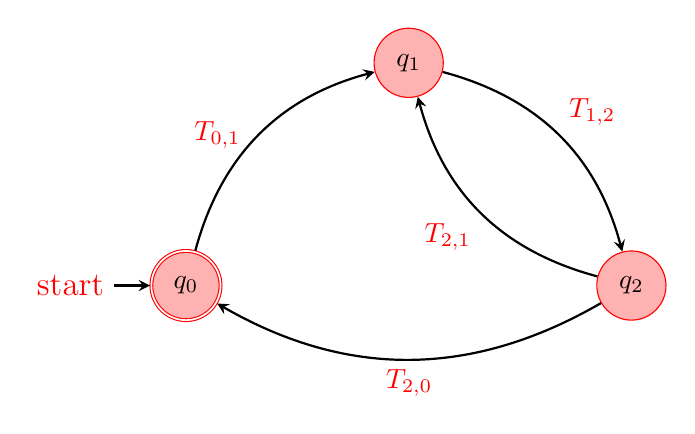
\begin{tikzpicture} [node distance = 4cm, on grid, auto,every state/.style = {draw = red, fill = red!30},
every initial by arrow/.style = {font = \large, text = red, thick,-stealth}]

% States
\node (q0) [state, initial, accepting, initial text = {start}] {$q_0$};
\node (q1) [state, above right = of q0] {$q_1$};
\node (q2) [state, below right = of q1] {$q_2$};

% Transitions
\path [-stealth,thick,text=red]
	(q0) edge [bend left]  node [left=0.1cm] {$T_{0,1}$}    (q1)
  (q1) edge [bend left]   node[above right]         {$T_{1,2}$}    (q2)
	(q2) edge [bend left]   node[below]         {$T_{2,0}$}  (q0)
	(q2) edge [bend left]   node[below left]         {$T_{2,1}$}    (q1);
\end{tikzpicture}

\end{document}